\section{Approach}
To schedule processing tasks on software defined networks, we identified two approaches, which we
named \textit{Top-Down} and \textit{Bottom-Up}. A sketch of these concepts and their relation to the
setup is depicted in Figure \ref{fig:schedulingapproaches} and described in the following section.

\begin{figure}[h]
    \centering
    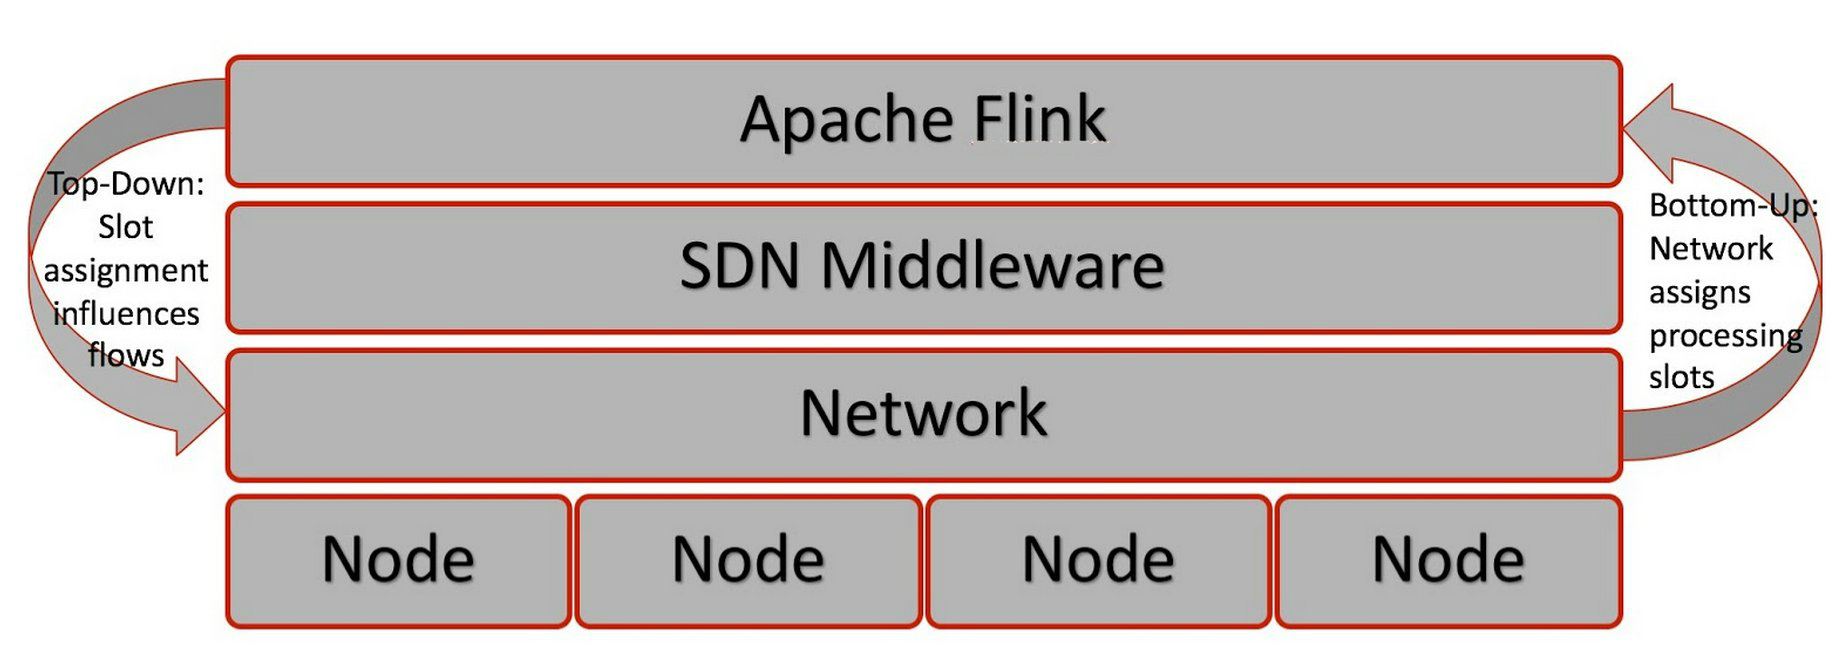
\includegraphics[width=0.75\textwidth]{graphics/schedulingapproaches.png}
    \caption{Different scheduling approaches}
    \label{fig:schedulingapproaches}
\end{figure}

We make the following assumptions:
\begin{itemize}
\item Jobs are not scheduled in parallel but one after another. Otherwise, the scheduler may
interfere with scheduling multiple jobs concurrently.

\item Jobs always communicate All-To-All. This holds true for the experiments conducted within this
paper and eliminates the need to traverse the execution graph. Also, this benefits the generic
approach since no deep Flink requirement is built up and the application can be more easily ported.

\item Due to the fact that network behaviour is to be studied, the focus lies on network
communication. If a single task manager offers multiple processing slots, network effects are
weakened. Therefore, a task manager consists of a single processing slot in our setup.
\end{itemize}

These constraints limit real-world applications but can easily hold true for our test setup to
determine performance gains with the concepts introduced.

\subsection{Top-Down/Flow Switching}
The \textit{Top-Down} approach imposes that the data processing engine schedules tasks as usual and
does not take network properties into account. The middleware is aware of these scheduling decisions
and influences the network properly. This influence could be either providing additional bandwidth
between communicating hosts through flow switching or limiting bandwidth on the specific
communication links for background activities. Advantages of this approach are that there is no
modification on the scheduler required and it is more portable since only a data processing
engine-middleware interface must be implemented. A major disadvantage is the possible worst case:
Parts of a job could be scheduled in a data center and another part far away like in another network
region.

\subsection{Bottom-Up/Scheduling}
The \textit{Bottom-Up approach} required the data processing engines' scheduler actively asks the
middleware for a node to place the task on. The middleware is aware of the network topology and can
determine optimal task placement through proper algorithms. The disadvantage of this approach is
that the data processing engines’ scheduler needs to be modified to interact with the middleware.
Advantages would be that the middleware is in full control of job placement what not only ensures
optimal placement but also can add optional constraints like only use certain network areas for
processing during maintenance etc.

A detailed description of the actual implemented algorithms used is given in section
\ref{sec:middleware_slot_assignment}.
